\documentclass[11pt,letterpaper]{article}
\usepackage[utf8]{inputenc}

%----- Configuración del estilo del documento------%
\usepackage[table]{xcolor}
\usepackage{epsfig,graphicx}
\usepackage[left=2cm,right=2cm,top=1.8cm,bottom=2.3cm]{geometry}
\usepackage{fancyhdr}
\usepackage{lastpage}
\pagestyle{fancy}
\fancyhf{}
\rfoot{\textit{Página \thepage \hspace{1pt} de \pageref{LastPage}}}


%------ Paquetes matemáticos básicos --------%
\usepackage{amsmath}
\usepackage{amssymb}
\usepackage{amsthm}

%------ Texto aleatorio ----- %

\usepackage{lipsum}
\usepackage{enumitem}


\begin{document}

%------ Encabezado -------- %

\begin{center}
    \begin{minipage}{3cm}
    	\begin{center}
    		\includegraphics[height=3.4cm]{./imagenes/logo_unam.png}
    	\end{center}
    \end{minipage}\hfill
    \begin{minipage}{10cm}
    	\begin{center}
    	\textbf{\large Universidad Nacional Autónoma de México}\\[0.1cm]
        \textbf{Facultad de Ciencias}\\[0.1cm]
        \textbf{Matemáticas para las Ciencias Aplicadas $|$ Grupo 7048}\\[0.1cm]
        \textbf{Tarea 4 }\\[0.1cm]
        Real Araiza Yamile\\[0.1cm]
        Rodríguez López Luis Fernando\\[0.1cm]
        Tenorio Reyes Ihebel Luro\\[0.1cm]
        25/11/2024
    	\end{center}
    \end{minipage}\hfill
    \begin{minipage}{3cm}
    	\begin{center}
    		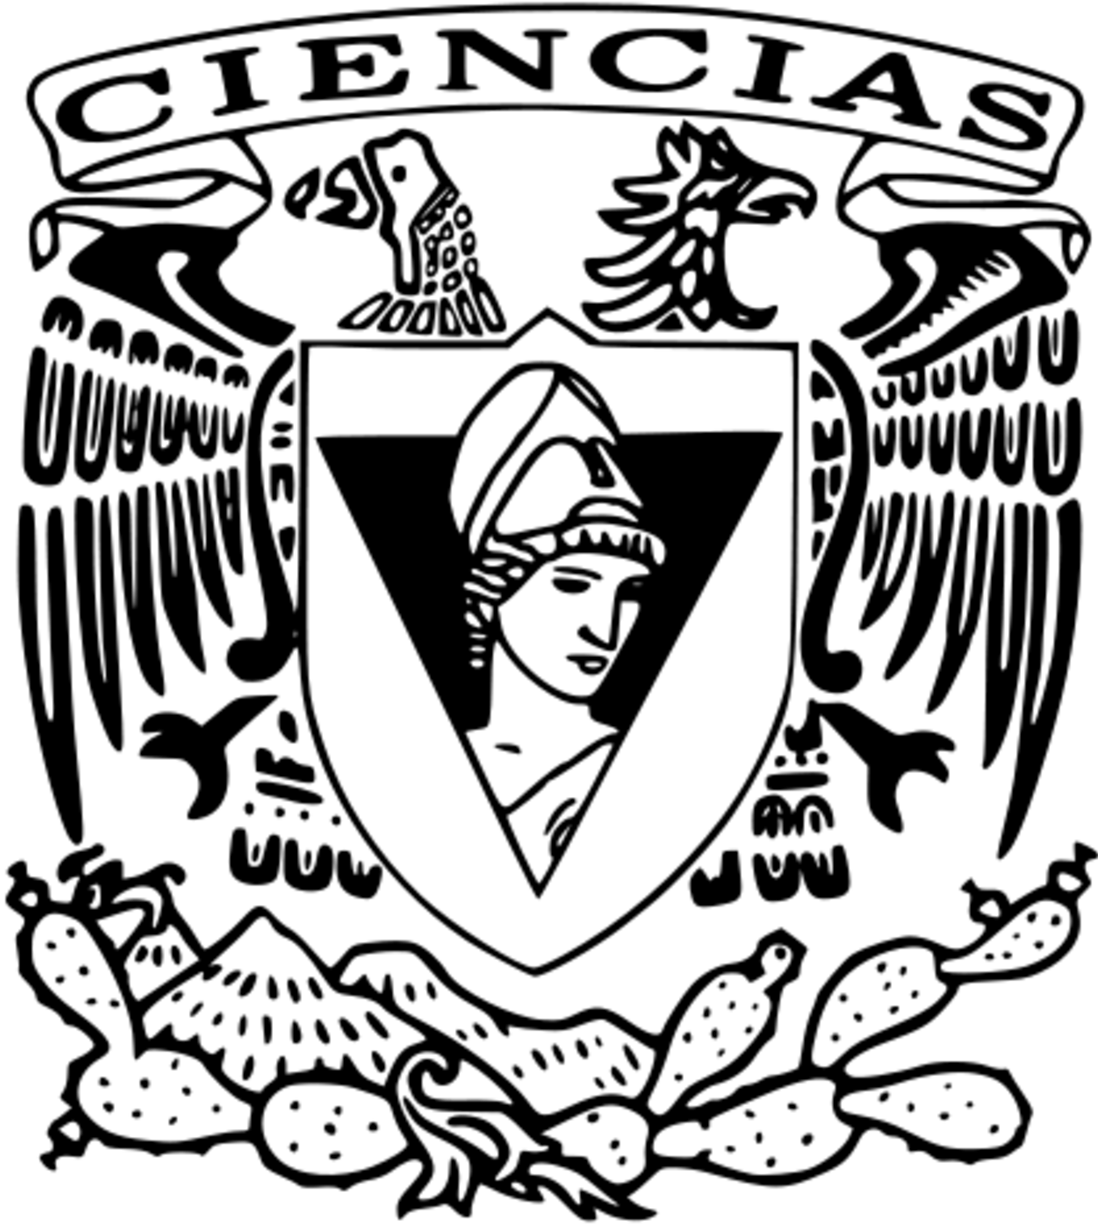
\includegraphics[height=3.4cm]{./imagenes/Logo_FC.png}
    	\end{center}
    \end{minipage}
\end{center}

\rule{17cm}{0.1mm}

%------ Fin de encabezado -------- %

%\section*{1ra Parte}

\subparagraph{Ejercicios: Review Exercises Capítulo 5 Anton-Bivens-Davis (pp. 408-412).}

% ---- 01. Ejercicio 13 IHEBEL ---- %
\section{Ejercicio 13, cap V Review Exercises.}

% ---- 02. Ejercicio 23 YAMILE ---- %
\section{Ejercicio 23, cap V Review Exercises.}

% ---- 03. Ejercicio 42 YAMILE ---- %
\section{Ejercicio 42, cap V Review Exercises.}

% ---- 04. Ejercicio 53 LUIS ---- %
\section{Ejercicio 53, cap V Review Exercises.}

% ---- 05. Ejercicio 56 LUIS ---- %
\section{Ejercicio 56, cap V Review Exercises.}

% ---- 06. Ejercicio 64 LUIS ---- %
\section{Ejercicio 64, cap V Review Exercises.}

% ---- 07. Ejercicio 68 IHEBEL ---- %
\section{Ejercicio 68, cap V Review Exercises.}

% ---- 08. Ejercicio 73 LUIS ---- %
\section{Ejercicio 73, cap V Review Exercises.}

% ---- 09. Ejercicio 76 YAMILE ---- %
\section{Ejercicio 76, cap V Review Exercises.}

% ---- 10. Ejercicio 85 IHEBEL ---- %
\section{Ejercicio 85, cap V Review Exercises.}



%\section*{2da Parte}

\subparagraph{Ejercicios: Review Exercises Capítulo 6 Anton-Bivens-Davis (pp. 485-486).}

% ---- 11. Ejercicio 7 YAMILE ---- %
\section{Ejercicio 7, cap VI Review Exercises.}

% ---- 12. Ejercicio 13 LUIS ---- %
\section{Ejercicio 13, cap VI Review Exercises.}

% ---- 13. Ejercicio 16 YAMILE ---- %
\section{Ejercicio 16, cap VI Review Exercises.}

% ---- 14. Ejercicio 19 IHEBEL ---- %
\section{Ejercicio 19, cap VI Review Exercises.}



\subparagraph{Ejercicios: Review Exercises Capítulo 7 Anton-Bivens-Davis (pp. 557-559).}

% ---- 15. Ejercicio 8 IHEBEL ---- %
\section{Ejercicio 8, cap VII Review Exercises.}

% ---- 16. Ejercicio 14 LUIS ---- %
\section{Ejercicio 14, cap VII Review Exercises.}

% ---- 17. Ejercicio 33 LUIS ---- %
\section{Ejercicio 33, cap VII Review Exercises.}

% ---- 18. Ejercicio 41 IHEBEL ---- %
\section{Ejercicio 41, cap VII Review Exercises.}

% ---- 19. Ejercicio 51 YAMILE ---- %
\section{Ejercicio 51, cap VII Review Exercises.}


% ---- 20. Ejercicio YAMILE ---- %
\section{Ejercicio: Classroom.}

\end{document}